\documentclass[11pt, conference]{IEEEtran}
\usepackage{xeCJK}
\usepackage{amsmath}
\usepackage{listings}
\usepackage{amssymb}
% 用来断词,当出现花括号中的单词时,若遇到换行需要断词的话就只能从-处断。
\hyphenation{op-tical net-works semi-conduc-tor}

\begin{document}
    \title{Report of Chapter 3: Model Checking}
    \author{\IEEEauthorblockN{林奇峰, Qifeng Lin}\IEEEauthorblockA{Student ID:17214656}}
    \date{\today}
    \maketitle

    \section{Review}
    In this chapter, it mainly demonstrates two methods to perform model checking. One is based on CTL and the other one on PLTL, which leads to independent development of them. And in my opinion, CTL is easier than PLTL to understand for which CTL provides direct codes to show how it runs. 
    
    The first one, CTL , can perform model checking in linear time in each component and reasons in terms of which state satisfies which formula. And the fundamental procedure of CTL is \textbf{marking}. CTL will mark each state the values of sub-formulas they hold. For example, \textbf{q.psi} is true if $q\models\psi$, otherwise \text{false}. After marking all the sub-formuals and formulas, we can easily to judge if $\mathcal{A}\models\phi$ by looking up the value of \text{q0.phi} of initial state $q_0$. Then, the crux of the algorithm is given as Figure 1 shows:
    

    For case 1, it just needs to mark if states hold the atomic proposition, true for yes and false for no.
    
    For case 2, it just needs to reverse the value of case 1.
    
    For case 3, it is the conjunction of two sub-formulas. After marking each sub-formulas then perform the operation "and".
    
    For case 4, it is also easier to understand. Because we need to find if the state which follows state $q$ satisfies $\psi$, we just check the value of its successors.
    
    For case 5, we need to check if there is an execution to verify that when a state satisfies $\psi_2$, $psi_1$ of all the predecessors including itself can be verified. Therefore, we firstly marking all the sub-formulas. Then, extract all the states that satisfy $\psi_2$. After that, we traverse back to their predecessors to find if they satisfy $\psi_1$. To avoid visited states repeatedly, set a boolean variable separately to keep track of its change. In this way, we can easily to judge whether current state satisfies $\phi$. 

    For case 6, we need to check if all the executions from current state satisfy $\phi$. Firstly, mark all the sub-formulas and then extract all the states that satisfy $\psi_2$. Since we need to check all executions, we choose to set a counter to record the number of successors that satisfy $\phi$, of current state. Compared with case 5, the most different point is the counter. But I can not understand why it set the value of $\phi$ of initial states that satisfy $\psi_2$, to true without checking $\psi_1$ of those. Therefore, it confuses me a lot and I think it needs to be corrected. 
    
    
    \begin{figure}
  \centering
  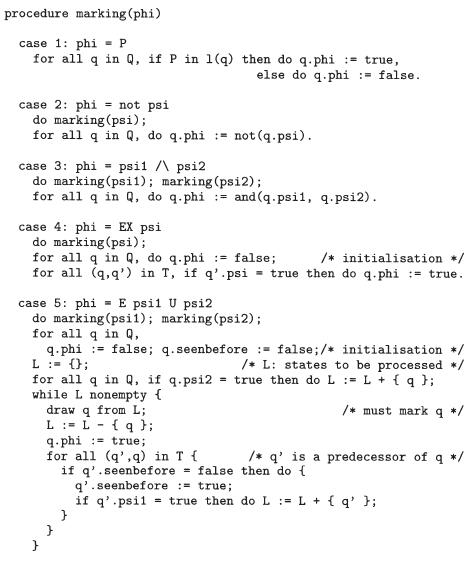
\includegraphics[width=3.0in]{1.jpg}
\end{figure}
\begin{figure}
  \centering
  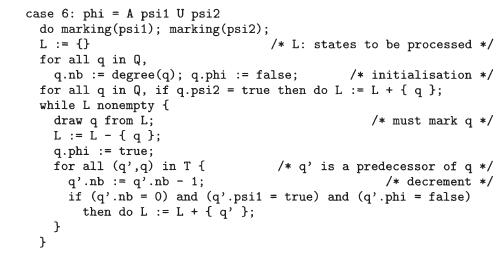
\includegraphics[width=3.in]{2.jpg}
  \caption{Six cases for CTL}
\end{figure}

    all cases above are easy to understand for which the codes are given out and it is very clear. And from above, it can be observed that the time required to perform CTL model checking is in $O(|Q|+|T|)$, that is, $O(|\mathcal{A}|)$. Because all the relevant operations are associated with either states $q \in Q$ or transitions of $T$.
    
    The second one is PLTL model checking. different from CTL, PLTL does not rely on marking states and it adopts a different viewpoint--language theory. It extends the well-known regular expressions to $\omega$-regular expressions. Compared with regular expression, $\omega$-regualr expression adds a new exponent "$\omega$" to mean infinite number. Though, it performs model checking on a automaton rather on a $\omega$-regular expression. Therefore, the most important procedure of PLTL is to construct an automaton $\mathcal{B}_{\neg\phi}$ to recognize the executions that do not satisfy $\phi$. 
    
    To explain principles of PLTL model checking, a simple example is given out. Firstly, giving a formula $\phi$:$\text{\textbf{G}}(P)\Rightarrow\text{\textbf{X}}\text{\textbf{F}}Q$, then an automaton $\mathcal{B}_{\neg\phi}$ is constructed as Figure 2 shows.
\begin{figure}
  \centering
  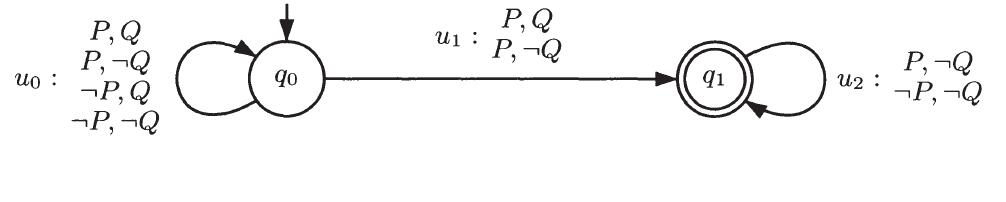
\includegraphics[width=3.0in]{3_1.jpg}
  \caption{$\mathcal{B}_{\neg\phi}$ for $\phi$:$\text{\textbf{G}}(P)\Rightarrow\text{\textbf{X}}\text{\textbf{F}}Q$}
\end{figure}
\begin{figure}
  \centering
  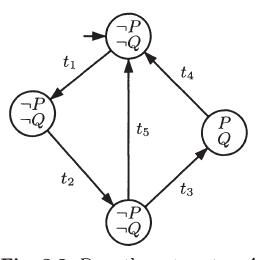
\includegraphics[width=2.0in,height=2.0in]{3_2.jpg}
  \caption{Does the automaton $\mathcal{A}$ verify $\phi$:$\text{\textbf{G}}(P)\Rightarrow\text{\textbf{X}}\text{\textbf{F}}Q$}
\end{figure}
    we can observe that the transitions of $\mathcal{B}_{\neg\phi}$ are labelled by propositions and if $q_0$ moves to $q_1$ is not deterministic. But once $\mathcal{B}_{\neg\phi}$ can remain in $q_1$ infinitely without blocking, then $\phi$ can not be satisfied because all transitions include only $\neg Q$. And we denoted the side where $\phi$ can not be satisfied as double circle. 
    
    After that, for automaton $\mathcal{A}$, it is given as Figure 3 shows.

\begin{figure}
  \centering
  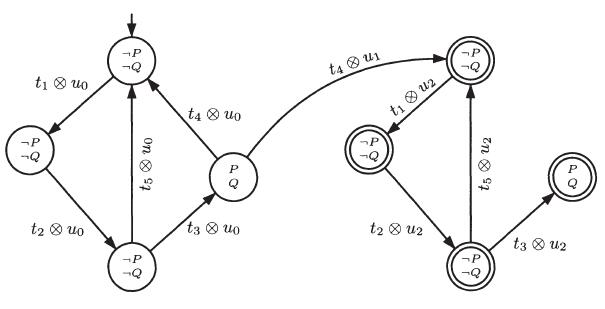
\includegraphics[width=4.0in]{3_3.jpg}
  \caption{The product $\mathcal{A}\otimes\mathcal{B}_{\neg\phi}$}
\end{figure}

    Though the automaton $\mathcal{A}$ is the origin object we want, we choose to apply the product of $\mathcal{A}$ and $\mathcal{B}_{\neg\phi}$ into $\mathcal{A}\otimes\mathcal{B}_{\neg\phi}$ by strongly synchronizing them. In this way, we can easily to know if the automaton $\mathcal{A}\otimes\mathcal{B}_{\neg\phi}$ remain in the side where double circle exists.
    
    Explain Figure 4 in detail. $t\otimes u_1$ happens if and on if it leaves from a state that satisfies $P$, that is $l(q)=\{P,Q\}$ or $l(q)=\{P\}$. $t\otimes u_2$ happens if and only if it leaves from a state that satisfies $\neg Q$, that is $l(q)=\{P\}$ or $l(q)=\{\}$. Therefore, $\mathcal{A}\otimes\mathcal{B}_{\neg\phi}$ only has 10 transitions instead of the theoretical maximum of 5x3.
    
    Then, back to the Figure 4, we can observe that from initial state, $\mathcal{A}\otimes\mathcal{B}_{\neg\phi}$ is possible to evolve to double circle side through $t_4\otimes u_1$, where it will 
    remain indefinitely. it means that the language recognized by $\mathcal{A}\otimes\mathcal{B}_{\neg\phi}$ is not empty and therefore $\mathcal{A} \nvDash \phi$ .
    
    As for the complexity of PLTL, it can be given as following:
    \begin{itemize}
      \item $\mathcal{B}_{\neg\phi}$ has size $O(2^{|\phi|})$ in the worst case;
      \item the product $\mathcal{A}\otimes\mathcal{B}_{\neg\phi}$ has size $O(|\mathcal{A}|\text{x}|\mathcal{B}_{\neg\phi}|)$
      \item if $\mathcal{A}\otimes\mathcal{B}_{\neg\phi}$ fits in computer memory, we can determine whether it accepts a nonempty language in time $O(|\mathcal{A}\otimes\mathcal{B}_{\neg\phi}|)$
    \end{itemize}
    
    Though two methods are introduced to perform model checking, state explosion problem is unavoidable for which they all rely on the explicit construction of the automaton $\mathcal{A}$. For CTL, it needs to traversal and markings and for PLTL, it needs to construct the automaton $\mathcal{B_{\neg\phi}}$ and the synchronizes with  $\mathcal{B_{\neg\phi}}$ by seeking of reachable states and loops. Therefore, it needs other methods to solve state explosion problem
    
    \section{Summary}
    This chapter introduce how to use CTL and PLTL to perform model checking. The easiest to understand is CTL for which all steps can be reasoned by scanning codes. PLTL checks the model mainly through constructing the automaton $\mathcal{B_{\neg\phi}}$ and synchronizing with it. And the common disadvantage of both methods is state explosion problem.
\end{document} 